\chapter{Doug Williams: Focus, Scale, and the Risk Meter}

This interview is not a blackboard lecture, but it has a definite quantitative spine. Doug Williams moves from capital allocation to operating focus, from selling to scaling, and then from career durability to risk judgment. The numbers are few but important: a $50 million venture pool, early checks in the range of $500,000 to $2$-$3 million, portfolio companies often below $2 million in revenue, five and a half million American miles, and an HMS Holdings sale reported at $3.5 billion. We will treat those figures as anchors, and we will treat the rest of the lecture as a study in how judgment, preparation, and alignment turn capital into operating progress.

\section{Credentials, Capital, and the Investor's Filter}

Williams is introduced through a concrete career claim: he was formerly chief operating officer of HMS Holdings, a healthcare company sold for about $3.5 billion. The point of the opening is not biography for its own sake. It establishes that the advice which follows comes from someone who has operated inside a company large enough to matter, sold into large organizations, sat on boards, and now allocates capital to early-stage companies.

The first question asks what he looks for when investing. He answers with scale and stage before he answers with philosophy. The venture vehicle has about
\begin{equation}
C \approx \$50{,}000{,}000
\end{equation}
available to invest. The rounds are early, and a typical investment is roughly
\begin{equation}
I \in [\$500{,}000,\ \$2{,}000{,}000\text{ to }\$3{,}000{,}000].
\end{equation}
The companies are usually not mature operating machines. They are often generating less than about
\begin{equation}
R \lesssim \$2{,}000{,}000
\end{equation}
in revenue.

That stage explains the filter. Williams looks for interesting ideas, thoughtful management teams, and large target markets. But the investor's work does not stop at the check. The companies then need organization, talent, and focus. In this lecture, venture capital is not merely money placed on a table. It is money plus repeated intervention on where the company should aim.

A compact way to write the filter is
\begin{equation}
\text{Investable company}
\approx
\text{idea}
+
\text{team}
+
\text{large market}
+
\text{focus}.
\end{equation}
This is not a formula Williams writes down. It is a note-writing shorthand for the sequence in his answer.

\section{Focus as the Investor's Operating Role}

Williams next shifts from what he funds to what he does after funding. Young CEOs, he says, can have too many things coming at them and too few people to handle them. The operating problem is not only lack of capital. It is lack of discrimination among competing demands.

He describes his role as coaching CEOs, direct reports, and boards toward the right target. The sectors he names are behavioral health and digital health, with examples including concussion monitors, anxiety-related work for troops, and drug studies. The variety of companies matters because it gives the coaching problem a general form: the details differ, but the CEO still has to choose what matters now.

We can express the coaching rule as a filtering operation. Let \(A\) be the set of all possible actions confronting the CEO, and let \(A^\ast\) be the small set of actions that are actually high impact:
\begin{equation}
A^\ast = \{a \in A : a \text{ is focused, timely, and material to the company}\}.
\end{equation}
The board member's practical contribution is to help the CEO move from the noise of \(A\) to the narrower set \(A^\ast\). This is the first recurring motif of the interview: focus is a form of leverage.

\section{Selling Through Consequence, Not Hype}

The interviewer asks for a specific coaching example, and Williams gives one. He describes a smart founder who understood the market and the product, but whose message would not land. The problem was not intelligence. It was translation into buyer consequence.

Williams's phrase is that one sells through fear, not foresight. He does not mean panic or manipulation. He means that the buyer often responds more concretely to the risk of failure than to a vague promise of success. A CEO is not mainly afraid of being too successful. The CEO is afraid of failing in a way that damages the business.

\subsection{Question \& Answer}

\paragraph{Question.}
Why would a seller emphasize fear of failure rather than the upside of success?

\paragraph{Answer.}
Because the buyer's immediate problem is usually not an abstract future benefit. It is a present vulnerability. If the seller can show, truthfully and specifically, that ignoring the problem will hurt the buyer's business, then the buyer has a reason to act. The message becomes: here is the business failure this product helps you avoid.

The same section introduces credibility. Williams points out the dynamic of a small company selling to a much larger one. His example is a company around $2 million in size trying to sell into a $50 billion company. The size gap creates a trust problem:
\begin{equation}
\text{seller scale} \ll \text{buyer scale}.
\end{equation}
In that situation, credibility can be borrowed from a trusted intermediary. If the large buyer already trusts Williams, then some of that trust can transfer to the young company he is bringing forward. That trust was not created in the moment. It was accumulated over years in the market.

\section{Solution Selling: Let the Buyer Buy}

The next question asks how someone can ``crush sales.'' Williams's answer begins with a distinction: no one likes to be sold to, but everybody likes to buy. The sales process is therefore not a performance in which the seller shows everything and hopes something sticks. It is a diagnostic process.

The order matters:
\begin{enumerate}
\item Do homework before the meeting.
\item Ask questions before showing the product.
\item Understand the true need.
\item Identify the buyer's pain points.
\item Offer a mutual solution.
\end{enumerate}
This reverses the demo-first habit of many inexperienced sellers. In a demo-first sale, the seller starts with inventory: here is everything we can do. In Williams's method, the seller starts with the buyer's state: here is the problem you are actually trying to solve.

A concise update rule for the sales conversation is
\begin{align}
\text{homework} &\longrightarrow \text{questions},\\
\text{questions} &\longrightarrow \text{true need},\\
\text{true need} &\longrightarrow \text{pain point},\\
\text{pain point} &\longrightarrow \text{mutual solution}.
\end{align}
The important word is ``mutual.'' The seller is not simply trying to close a transaction. The seller is trying to make the buyer's own decision clear enough that buying becomes the natural act.

\begin{figure}
\centering
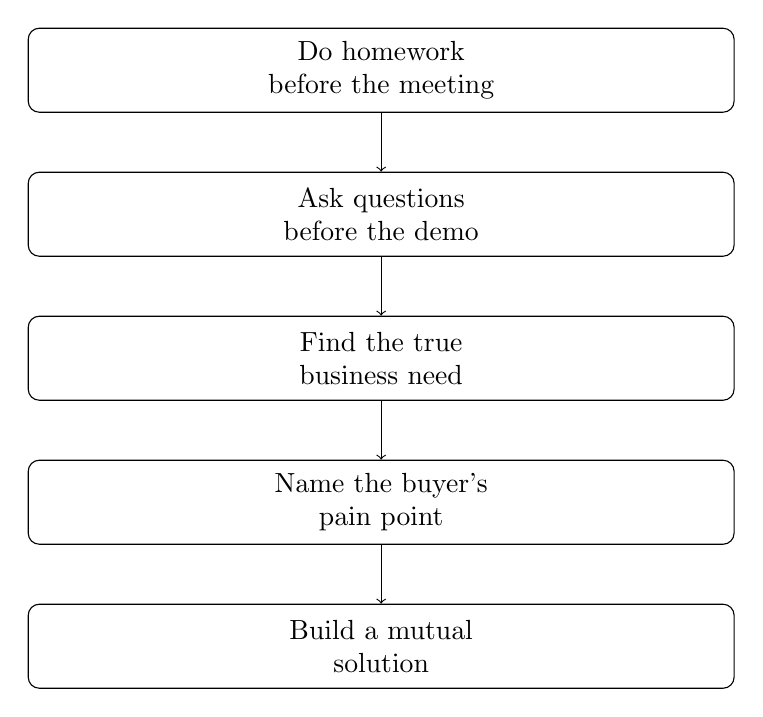
\begin{tikzpicture}[
  box/.style={draw, rounded corners, align=center, text width=0.72\linewidth, minimum height=0.42in},
  node distance=0.72in
]
\node[box] (a) {Do homework\\before the meeting};
\node[box, below of=a] (b) {Ask questions\\before the demo};
\node[box, below of=b] (c) {Find the true\\business need};
\node[box, below of=c] (d) {Name the buyer's\\pain point};
\node[box, below of=d] (e) {Build a mutual\\solution};
\draw[->] (a) -- (b);
\draw[->] (b) -- (c);
\draw[->] (c) -- (d);
\draw[->] (d) -- (e);
\end{tikzpicture}
\caption{Transcript-backed reconstruction of Williams's solution-selling sequence.}
\end{figure}

\section{Scaling as a Designed Doubling Playbook}

The interviewer then asks how a business scales from six figures to seven, eight, and beyond. Williams begins with valuation language: companies are often sold from a multiple of revenue or EBITDA. The transcript does not give a specific multiple, so the safe notation is only a shorthand:
\begin{equation}
V \approx m_R R
\qquad\text{or}\qquad
V \approx m_E E,
\end{equation}
where \(R\) is revenue, \(E\) is EBITDA, and \(m_R,m_E\) are market multiples not specified in the interview. The HMS sale itself is simply reported as
\begin{equation}
V_{\mathrm{exit}} \approx \$3.5\text{ billion}.
\end{equation}

Then Williams turns from valuation to operations. To scale, he says, one has to get the basics right: value proposition, total addressable market, buyer, and key message. Only after those basics are clear does the wheel begin to spin.

His main image is a folding piece of paper. He plans the company where it is today, then asks what happens when it doubles, and then what happens when it doubles again. If \(S_0\) denotes the present scale, the reconstruction is
\begin{equation}
S_n = 2^n S_0.
\end{equation}
This is not a board equation. It is the mathematical skeleton of the verbal doubling model.

\subsection{Question \& Answer}

\paragraph{Question.}
What has to be designed before a company scales?

\paragraph{Answer.}
Not only the product. Williams names organizational structure, metrics, alignment, relationships, and channels. If those are designed before the next doubling, the company does not have to improvise every time growth arrives.

\begin{figure}
\centering
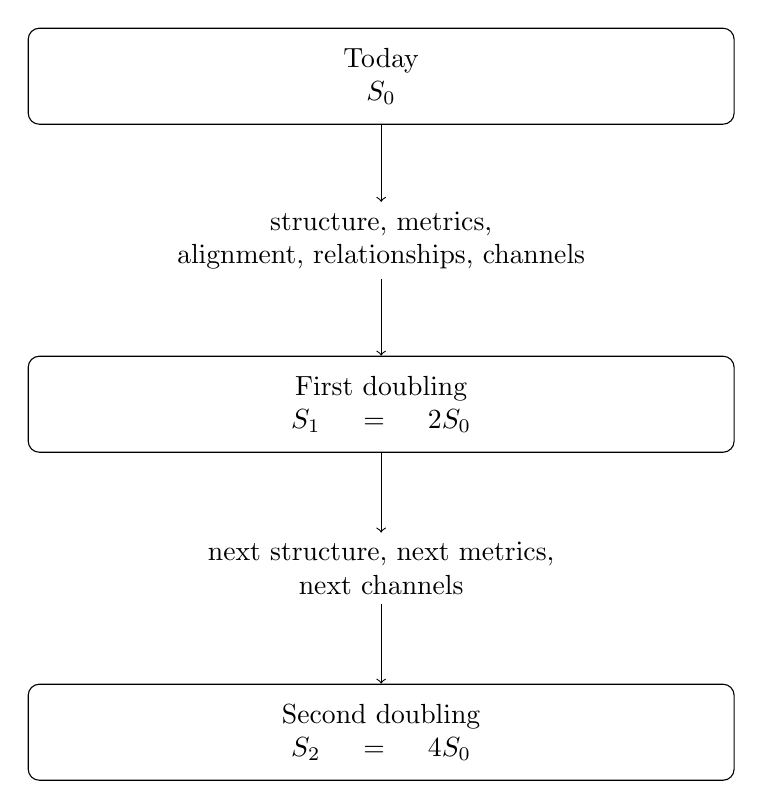
\begin{tikzpicture}[
  stage/.style={draw, rounded corners, align=center, text width=0.72\linewidth, minimum height=0.48in},
  small/.style={align=center, text width=0.72\linewidth},
  node distance=0.82in
]
\node[stage] (s0) {Today\\\(S_0\)};
\node[small, below of=s0] (p0) {structure, metrics,\\alignment, relationships, channels};
\node[stage, below of=p0] (s1) {First doubling\\\(S_1=2S_0\)};
\node[small, below of=s1] (p1) {next structure, next metrics,\\next channels};
\node[stage, below of=p1] (s2) {Second doubling\\\(S_2=4S_0\)};
\draw[->] (s0) -- (p0);
\draw[->] (p0) -- (s1);
\draw[->] (s1) -- (p1);
\draw[->] (p1) -- (s2);
\end{tikzpicture}
\caption{A narrow reconstruction of the scaling-by-doubling playbook.}
\end{figure}

The payoff is speed. If the plan already exists, raising more money, using a banking relationship, or adding leverage has a frame around it. Scaling by design is faster than simply doing more and more of the same thing.

\section{Career Durability and the Cost of Money Alone}

The interview then pivots to Williams's book, \emph{Shift: A Playbook for Positive Change}. He says the working title had been something like \emph{Enjoy the Walk} or \emph{Enjoy the Journey}. The lesson is not that titles matter. It is that a career is partly remembered through the skills learned and the people met along the way.

This section widens the meaning of entrepreneurship. Success is not only the company, the job, or the exit. Williams emphasizes mentors, people one works with, helping others get better, and helping people move up even if they eventually leave one's direct orbit. The mechanism is not sentimental. The human network is part of long-run capability.

The next question is about work-life balance. Williams calls it a tough question, then gives concrete operating boundaries. He had five and a half million American miles, so travel was heavy:
\begin{equation}
M_{\mathrm{travel}} \approx 5.5\text{ million miles}.
\end{equation}
But he says that when he was away from home, he worked, and when he came home, he was home. He avoided calls all day Saturday. After everyone went to bed Sunday, he might spend an hour or an hour and a half preparing for the week. The principle is separation by context:
\begin{equation}
\text{away} \mapsto \text{work},
\qquad
\text{home} \mapsto \text{family}.
\end{equation}

The warning is sharp. A person can work hard, accumulate money, retire at 65 or 70, and discover that the relationships, friends, and family network were never built. Money by itself is not the end state the entrepreneur imagined.

\section{Mental Balance and Transferable Skill}

The mental-health question keeps the same logic but makes it more personal. Williams says one must have more than one focus in life. His rhythm is concrete: up at 4:30, in the gym by 5, generally working out seven days a week. Some days include more than one workout. The exercise is not merely fitness; it is mind space.

His hobbies continue the same pattern: golf, sailing, hiking, and road biking. He invokes the Abraham Lincoln sharpening-the-ax story as a way of naming renewal before action. The practical proposition is that stress falls when a person is trained, prepared, and not living in a pressure cooker all the time.

The interview then returns to career path. Williams began as a computer programmer. In his first job, he programmed devices, worked on B-1 bombers, worked on Disneyland systems, and learned how devices talk to each other. The important transferable skill was not syntax alone. It was protocols, field work, companies, and people.

That field exposure led to Arthur Andersen, where he became a partner, then healthcare technology leadership, healthcare IBM consulting worldwide, and eventually HMS Holdings. The opening credential now returns as the end of a path:
\begin{equation}
\text{programming}
\longrightarrow
\text{field problems}
\longrightarrow
\text{consulting}
\longrightarrow
\text{healthcare operations}
\longrightarrow
\text{HMS}.
\end{equation}
The chapter should read this as compounding. Technical skill becomes commercial skill when it is repeatedly tested against real organizations and real users.

\section{Risk, Due Diligence, and Helping Others}

The final movement begins with financial decisions. Williams jokes that his worst decision was not buying enough Bitcoin or Tesla. More seriously, he says he has lost money on an investment, but when he looked back at the data and the people at the time, he still thought it was a good bet. That distinction matters: a bad outcome is not automatically a bad decision.

His risk principle is qualitative:
\begin{equation}
\text{perfect success rate}
\quad\Rightarrow\quad
\text{risk meter may be too low}.
\end{equation}
This is not a probability model. It is a warning that avoiding every loss may also mean avoiding the level of uncertainty required for meaningful upside.

The practical due-diligence rule is to know people before investing with them. Not just through a demo or a PowerPoint presentation. Meet them, talk to them, get offline, and understand character. No business plan goes off flawlessly, so the investor wants to know how the people behave when the plan is no longer perfect.

We can write the due-diligence ladder as
\begin{equation}
\text{deck}
\longrightarrow
\text{conversation}
\longrightarrow
\text{context}
\longrightarrow
\text{character}
\longrightarrow
\text{alignment}.
\end{equation}
The last term is alignment. On boards, and among people brought in to help companies, Williams wants shared respect and a shared goal: make the play successful, not be the brightest light in the room.

The closing advice to Gen Z completes the pattern. Ask what you can do to help, not only what you can do to get ahead. Look for situations where you can lift someone else up. The commercial reason is that a reputation for helping becomes a form of accumulated trust. The human reason is simpler: if one builds a career alone, one should not be surprised to end up alone.

\section{Summary}

The lecture's center of gravity is disciplined judgment. Williams begins with capital, but the lesson is not that capital alone builds companies. Early-stage investing requires a filter: idea, team, market, stage, focus, and talent. Selling requires buyer diagnosis rather than performance. Scaling requires a predesigned doubling playbook. Career durability requires relationships, family boundaries, health, and skill renewal. Risk requires enough uncertainty to matter, but also enough due diligence to know the character of the people taking the risk with you.

The mathematical content is deliberately modest, because the source is an interview rather than a blackboard derivation. Still, the chapter has a quantitative frame: \(C \approx \$50{,}000{,}000\), \(I\) in the early-stage check range, \(R \lesssim \$2{,}000{,}000\), valuation by revenue or EBITDA multiple, and staged scale \(S_n=2^nS_0\). Those symbols are useful only if they serve the interview's main claim: entrepreneurship is not merely growth. It is growth under focus, credibility, preparation, alignment, and risk fit.